\documentclass{report}

\usepackage[utf8x]{inputenc}  % accents
\usepackage{geometry}         % marges
\usepackage[francais]{babel}  % langue
\usepackage{graphicx}         % images
\usepackage{verbatim}         % texte préformaté


\title{Rapport de Projet Hubosans4++} 
\author{Lucas BOURNEUF \&\& Thomas HUBA}
\date{9 janvier 2013}


% BEGIN
\begin{document}
\maketitle


%%%%%%%%%%%%%%%%%
% INTRODUCTION  %
%%%%%%%%%%%%%%%%%
\chapter*{Introduction}
    \paragraph*{}
        Le projet Hubosans4++ consiste en la réalisation d'un programme compilé avec gcc, permettant à un ou plusieurs utilisateurs de jouer à une variante du puissance 4, nommée le hubosans4++,
        apportant notamment le support de 2 à 6 joueurs et 3 types de pièces. 
    \paragraph*{}
        Les règles du jeu sont comparable à un puissance 4, si ce n'est que les pièces alignées ne doivent pas nécessairement être de même type, et qu'à chaque tour le joueur choisis, 
        en plus de la colonne, quel type de pièce lâcher. Les trois types de pièces ont chacune leur utilité : les pièces creuses et pleines se supperposent, 
        n'interfèrent pas les unes aux autres sinon pour réaliser un puissance 4 et ainsi gagner la partie. 
        Le troisième type, les pièces bloquantes, bloque littéralement une colonne en empêchant toute pièce de passer. La pièce bloquante est en fait la pièce du puissance 4 originel.
    \paragraph*{}
        Le jeu exploite la sortie et l'entrée standard : le couple écran/clavier, avec affichage dans le terminal d'où le jeu est lancé.
        Le jeu peut être sauvegardé pour être repris plus tard.
    \paragraph*{}
        Le jeu propose également le jeu contre une IA se contentant de cups au hasard. Une version plus élaborée, et bien plus intéressante, n'a n"anmoins pas été développée
            suffisemment rapidement pour intégrer le produit final du projet.



%%%%%%%%%%%%%%%%%
% ORGANISATION  %
%%%%%%%%%%%%%%%%%
\chapter{Organisation}
    \paragraph*{}
    Le projet étant divisés en modules les plus indépendants possible (architecture vue-contrôleur), les tâches ont été réparties selon un découpage logique.
    \paragraph*{}
    Ainsi, Lucas BOURNEUF s'est occupé de l'IA, de l'affichage dans la sortie standard, de la gestion mémoire et de l'interfaçage entre les modules. 
    Thomas HUBA s'est occupé des traitements du moteur et des sauvegardes.
    \paragraph*{}
    Un serveur git, hébergé sur github (https://github.com/Aluriak/Hubosans4), a été utilisé tout au long du projet (et ce fût la première chose proposée et mise en place dans ce projet) 
    pour assurer une gestion des version la plus efficace possible.\\
    Au fur et à mesure du projet, une documentation des fonctions principales de chaque modules a été écrite, dans le but de centraliser les primitives d'accès de chacun d'entre eux.

        \vspace{1cm}
        \begin{center}
            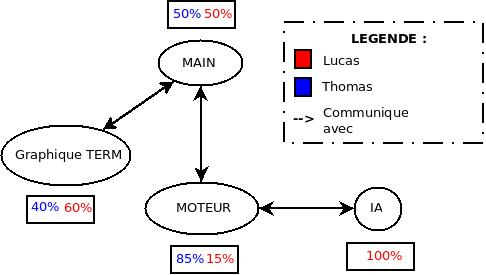
\includegraphics[width=10cm, height=6cm]{ressources/presentation/archi_projet.jpeg} \\
            \textbf{Figure 1 :} Architecture globale du projet, avec les principaux modules entrant en jeu.
        \end{center}

%%%%%%%%%%%%%%%%%
% ANALYSE       %
%%%%%%%%%%%%%%%%%
\chapter{Analyse}

    % % % % % % % % % % % %
    % Structures de données
    % % % % % % % % % % % %
    \section*{Structures du données}
        \paragraph*{}
        Les structures de données majeures sont la structure de jeu, de case, de joueur, et la pile d'action.
        \begin{itemize} % liste des structures de données principales
            \item la structure de jeu définit tout le reste, dans le sens où elle contient le plateau de jeu, simple matrice de case, la liste des joueurs et la pile d'action.
            \item la case contient quelques informations d'importance : les pièces présente dans la case et les id des joueurs les contrôlant
            \item les joueurs sont principalement définis par un nom, un nombre de points et un id unique permettant de les identifier rapidement.
            \item l'action est la structure de données principale de communication entre le moteur et les autres modules. Elle transmet toute les infos entre moteur et entrée utilisateur,
                ou encore l'IA.
            \item la pile d'action empile toutes les actions de jeu créé par les joueurs, humains ou IA. Ainsi, il est fort simple de revenir plusieurs coups en arrière, 
                ou d'effectuer le parcours d'arbre nécessaire à l'IA.
        \end{itemize}
        \paragraph*{} % MOTEUR
        Le moteur fait appel à beaucoup de structures de données, et certaines d'entre elles, notamment la structure de jeu, sont exploitées par beaucoup de modules. \\
        La structure de jeu, ou plutôt son adresse, est très souvent manipulée et envoyée à de nombreuses méthodes de modules. Contenant la totalités des valeurs du jeu, il paraît évident
        qu'elle soit nécessaire pour tout traitement sur celui-ci. Néanmoins, une règle n'est jamais enfreinte : seul le moteur \textbf{modifie} la structure. Tous les autres modules ne
        font que lire et interpréter le jeu. \\
        Ainsi, l'entrée utilisateur ou l'IA, même s'il reçoivent le jeu, ne font qu'interpréter ce dernier au mieux pour permettre à 
        l'utilisateur ou à l'ordinateur de choisir une colonne et un type de pièce. Ce choix est convertit en action, puis renvoyé à l'interface entre le moteur et le module, 
        qui transmettra l'action au moteur. C'est ce dernier qui interprètera l'action et effectuera les traitements nécessaires pour qu'elle soit prise en compte dans le jeu. 

        \paragraph*{} % PLATEAU DE JEU CASE
        Le plateau de jeu est une simple matrice de case, dont la taille, définie selon le nombre total de joueurs (6*7, plus une ligne et une colonne par joueur au-delà de deux), 
        est allouée dynamiquement. Les cases sont des structures fort simples, décrivant les joueurs contrôlant la case, et le type de pièce qu'elle contient.
        Ainsi, grâce à l'utilisation de l'id des joueurs, et d'une énumération explicitant le type de pièce (creuse, pleine, bloquante, double (pour creuse+pleine), ou vide), il est très
        simple de réaliser des études de la situation du plateau de jeu.

        \paragraph*{} % JOUEUR
        La liste de joueur contenue dans la structure de jeu est en réalité un tableau dynamique où sont indexés les joueurs. D'abords créés dans un ordre prévisibles, les joueurs voient
        le tableau mélangé, et reçoivent leur id, qui correpsond à leur index dans le tableau. Les id vont donc de 0 à 5 (6 joueurs maximum), et permettent l'accès direct à un joueur.\\
        Un joueur possède quelques attributs intéressants, notamment son score, son nom, sa réserve de pièce, son niveau d'IA.
        \begin{itemize} % liste des attriuts d'intérêt d'un joueur
            \item le score du joueur n'a pas d'influence réelle sur le jeu. Les joueurs humains pourront néanmoins prendre plaisir à optimiser leur scores au fil des parties.
            \item le nom du joueur, prédéfinit pour les IA, mais au choix pour les humains.
            \item la réserve de pièces restantes, autant en pièces bloquantes qu'en pleines ou creuses. 
            \item le niveau d'IA. S'il n'a aucun intérêt pour un joueur humain, le niveau d'IA est propre à chaque joueur IA et permet ainsi de faire joueur des IA de niveaux différents
                dans une même partie.
        \end{itemize} 
        \textit{Nota Bene} : un simple booléen est utilisé pour faire la différence entre un joueur humain et une intelligence artificielle. Les humains possède un niveau d'IA 
            positionné à la difficulté maximum.

        \paragraph*{} % PILE D'ACTIONS
        La pile d'action est une simple pile de structure d'action. Elle gère l'empilage, le désempilage, et sait à nimporte quel moment combien d'action elle contient. La mise en oeuvre
        de cette pile s'est implémentée par pointeur, pour des raisons de simplicité et d'efficacité. Elle permet de compter le nombre de tours déjà passés, (nombre d'actions contenues),
        de gérer facilement les retours en arrière (annulation de coup), \textit{et cetera}. \\
        La pile d'action du jeu ne contient que des actions de coup joué; les actions utilisateurs telles que la sauvegarde ou le retour au menu n'y sont pas empilés.

        \paragraph*{} % OYA
        Une autre donnée d'importance est l'oya. L'oya est le nom donné au joueur dont c'est le tour. Il est identifié par son id, permttant un accès direct à l'oya, 
        mais aussi aux joueurs suivants et précédents.

        \paragraph*{} % INTELLIGENCE ARTIFICELLE
        Pour l'IA, les même structures de données sont mises en oeuvre, puisqu'elles suffisent à l'exploration de l'arbre des possibilités. Néanmoins, le jeu est intégralement recopié
        dans la mémoire; il est en effet hors de question de laisser un autre module que le moteur modifier le véritable jeu. C'est sur cette copie du jeu que seront effectués 
        tous les traitements de parcours de l'arbre et de calcul de priorité d'une situation. 


    % % % % % % % % %
    % Fonctionnalités
    % % % % % % % % %
    \newpage
    \section*{Fonctionnalités} % (3 page min)
        \paragraph*{}
        \paragraph*{} %  entrée utilisateur
	Nous dissocierons 2 choses : \\
	\begin{itemize} % liste entrée menu & in_game
		\item Les entrées menus.
		Dans ce premier cas, c'est le main qui appel les procédures de graphique TERM. Celles-ci retourneront les valeurs entrées par l'utilisateur, le tout via regleJeu.nbJoueurs. En fonction de sa valeur, le main lancera les différentes procédures.\\
		Ainsi, la totalité des modules restent indépendant, l'un peut être modifié sans que l'on ait à changer quoique ce soit dans les autres modules. Ce principe est encore plus utile lors des parties en cours. 
		\item Les entrées utilisateurs dans une partie en cours.
		C'est la que la séparations des modules est la plus intéressante. En effet, le moteur est totalement indépendant du reste du programme. Celui-ci ne fait que reçevoir les données de graphique TERM. 
		Une fois les données reçues, le moteur les traite les données. Deux choix sont alors possible : \\
		\begin{itemize} % liste choix in_game
			\item Soit il s'agit d'une pièce que l'utilisateur veut placer. Dans ce cas, le moteur la reçois, test si celle-ci est possible à placer. Si oui, il modifie le plateau et passe l'oya au joueur suivant. 
			\item Soit il s'agit d'une commande dans le jeu. Par exemple, si l'utilisateur veut quitter, sauvegarder, annuler le dernier coup effectué, ou bien afficher l'aide des commandes. En fonctions de la valeurs reçue, le moteur retourne des valeurs spécifiques de GAGNANT (int retourné par le moteur) qui seront interprétées par le main.\\
                \end{itemize}
        \end{itemize}
	
	L'indépendance du MOTEUR est donc l'un des axes principaux sur lequel T.H. a travaillé.\\
		
        \paragraph*{} %- jeu contre IA
	Il est possible de jouer une partie contre une ou plusieur IA. Il est aussi possible de jouer uniquement contre des IA et de regarder la partie. 
	Plusieur niveau de difficulté sont présent : \\
	\begin{itemize}
		\item Facile : La profondeur de l'IA est faible (1 ou 2 coups d'avance) 
		\item Moyen : La profondeur de l'IA est un peu plus prononcer (3 coups d'avance) 
		\item Difficile : La profondeur de l'IA est grande (4 ou 5 coup d'avance) 
		\item Très Difficile : La profondeur de l'IA est maximale (l'IA voit jusqu'à la fin de la partie) \\
	\end{itemize}

        \paragraph*{} %- jeu à 6 joueurs
	Une des contraites imposées était de permettre un nombre de joueurs supérieur à 2.
	C'est ce que nous avons fait. Il est possible de jouer jusqu'à 6 joueur dans une même partie, IA ou HUMAIN confondu. 
	En principe il nous est possible de jouer jusqu'à 126 en même, mais le terminal à ses limites en taille et en couleur.
	En effet la taille est un problème évident, les proportions du plateau augmentant en fonction du nombre de joueur.
	Mais le nombre de couleurs disponible et reconnaissable par un humains sont limitées : nous avons jugé que seul 6 couleur pouvaient être suffisement reconnaissable.\\ 

        \paragraph*{} % sauvegarde
	En ce qui concerne la sauvegarde, aucun algorithme complexe n'était nécessaire. L'utilisateur ne peut sauvegarder qu'une partie en cours d'éxécution. Il s'agit donc d'une commande dans le jeu, c'est-à-dire que le moteur retour cette valeur au main, qui lancera le module de demande de slot à l'utilisateur. 
	Une fois cette valeur entrée, elle est retournée au main, qui rappellera le module sauvegarde du MOTEUR.
	C'est à ce moment là que le fichier de sauvegarde est crée (dans le répertoire SAVE), et que les données de jeu y sont enregistrées.\\
	
        \paragraph*{} % gestion des scores
	A chaque tour, la fonction de gestion des scores est lancée. En fonction de la dernière pièce jouée et de son id, les points du joueurs en cours sont modifié de la sorte : \\
	\begin{itemize}
		\item Si le joueur place une pièce PLEINE ou CREUSE sur une case VIDE = +30 points 
		\item Si le joueur place une pièce PLEINE ou CREUSE sur une case déjà occupée : +70 points 
		\item Si le joueur place une pièce BLOQUANTE : +20 points 
		\item Si le joueur bloque une suite de pièces adverse : \\
		\begin{itemize}
			\item Si la suite est de 2 pièces : +200 points 
			\item Si la suite est de 3 pièces : +300 points \\
		\end{itemize}
	\end{itemize}
	Afin de sécuriser les scores de toutes tentatives de modification volontaire et malhonnête, nous avons décidé de crypter le fichier des scores, et d'écrire plusieurs fois chaque données. Comme cela, on peut facilement déterminer si quelqu'un à voulu modifier au hasard (les données étant cryptées) les points ou les noms des joueurs. \\



    % % % % % % % % % %
    % Gestion d'erreurs
    % % % % % % % % % %
    \newpage
    \section*{Gestion d'erreurs} % (1 page min)
        \paragraph*{}
        Les principales sources d'erreur sont concentrées dans deux aspects du programme, tout deux liés intimement à l'utilisateur.\\
        Tout d'abord, l'entrée utilisateur, (navigations dans les menus, choix d'une pièce à mettre), et ensuite le chargement des sauvegardes.
        Une autre gestion d'erreurs interviendra lors des allocations dynamiques, pour éviter de grave problèmes de mémoire si jamais une allocation ne pouvait être réalisée.

        \paragraph*{} % entrée utilisateur
        L'entrée utilisateur est assurée par inSecure, un petit module dont le rôle principal est la capture d'un nombre et d'un mot dans une chaîne entrée par l'utilisateur, 
            dans l'entrée standard.
        Avec inSecure, la saisie est sécurisée (attaque par buffer overflow impossible), et efficace, puisque la méthode inSecure(int*, char*) est d'une simplicité d'utilisation
            à toute épreuve.
        Ainsi, les entrées utilisateurs sont protégées, si bien que ce dernier ne peut pas rendre l'execution du programme imprévisible par ce biais.

        \paragraph*{} % chargement des sauvegardes
        Le chargement des sauvegardes doit faire preuve d'une certaine rigeur. En effet, le MOTEUR doit à tout prix vérifier chaque valeur chargées, afin de ne pas dépasser la taille du plateau ou encore le nombre de joueurs autorisé. Nous pouvons ainsi vérifier en même temps si la sauvegarde n'est pas corrompue (on est vraiment jamais à l'abri d'une corruption de fichier).

        \paragraph*{} % allocations dynamique
        Le principe de la protection des allocations dynamique est fort simple : pour chaque allocation, une vérification est opérée. S'il s'avère que l'allocation a été refusée par l'OS,
        le programme est purement et simplement arrêté.

        \paragraph*{} % 
        Enfin, il est à noter que si la gestion d'erreur faite maison ne fonctionne pas, une assertion est utilisée et intercepte l'erreur au sein de la méthode FLUX\_ERREUR(2).
        Ainsi, même dans le cas où des erreurs se déclenchent dans le système de traitement d'erreur (notamment dans l'écriture des logs dans \textit{erreur.txt}), 
            le programme se terminera le plus proprement possible.


%%%%%%%%%%%%%%%%%
% CODAGE        %
%%%%%%%%%%%%%%%%%
\chapter{Codage} % (3 page min)
    \paragraph*{} % compilation séparée, makefile
    Le projet ayant dés le début été divisé en modules, un Makefile à été tenus à jour pour permettre une compilation efficace et simple; ainsi un simple \textit{make} suffit pour 
    compiler le projet et avoir le programme à jour, en évitant la compilation de smodules déjà à jour. \\
    De plus, \textit{make rapport} et \textit{make presentation} permettent quant à eux de générer respectivement le rapport de projet et la présentation. 
    Enfin, d'autres commandes ont été générées, notamment pour nettoyer le répertoire lors de mise à jour qui nécessitent la reconstrcution de l'entièreté des 
        fichiers intermédiaires et finaux.
    \paragraph*{} % notations
    Au sein du programme, la notation des fonctions suit une logique globale : les identificateurs des fonctions sont préfixés d'un signe d'appartenance à leur module, ou de la structure
        pour laquelle ces fonctions existent. Ainsi, nombreuses sont les fonctions commençant par \textit{MOTEUR\_}, ou bien \textit{t\_jeu\_}. Cela permet de bien montrer les frontères
        entre module et de clarifier l'utilisation de modules différents au sein d'une même méthode.
    \paragraph*{} % interfaçage
    Les modules sont interfaçés notamment dans le main, qui s'établis ainsi en code de haut niveau. On peut considérer que le projet à été réalisé en suivant une architecture 
        Modèle-Vue-Contrôleur, dans le sens où les différentes focntionnalités sont bien découpées les une des autres, et que les programmeurs ont tenté de les rendre les plus 
        indépendantes les unes des autres.
    \paragraph*{} % gestion de projet sous vim
    vim est l'éditeur de texte préféré des deux développeurs du projet, aussi a-t-il été utilisé massivement, à grand renforts de modules et bidouillages simplifiant la vie du projet, et
        faisant de vim un éditeur à part entière.
        \subparagraph*{} % modules
        Parmi les modules utilisé, on notera l'intégration de git au sein de vim (plus besoin de sortir de vim pour gérer les commit) avec \textit{fugitive}, quelques modules NERD, 
            notamment \textit{NERDcommenter} et \textit{NERDtree}, ou encore \textit{TeTrIs}, pour les pauses. \\
        Avec l'utilisation de la commande \textit{vim -c so\ projet.vim}, il est possible d'ouvrir tous les fichiers importants du projet, permettant en une commande d'avoir les 
            parties du projet les plus importantes à portée de clavier.\\
        Enfin, l'interfaçage très simple avec github au sein du terminal permettait d'être totalement indépendant de tout IDE.
    \paragraph*{} % algo notoires 
    Parmis les algorithmes notoires, on citera l'étude du jeu pour connaître la viabilité d'un puissance 4, ainsi que l'algorithme minimax mis en oeuvre pour l'IA.
    Ces deux algorithme sont choisis parce qu'il sont importants et utilisés souvent, ou, dans le cas de minimax, parce qu'il s'agit de l'algorithme le plus complexe du programme.
        \subparagraph*{} % puissance 4
	Afin de ne pas tester tout le plateau à chaque tour (solutions la plus facile mais la coûteuse en mémoire et en processeur), nous avons décidé de tester le puissance 4 juste après que la pièce est été posée par le joueur, et ce de la façon suivante : \\
	\begin{itemize}
		\item Test BAS - HAUT 
		\item Test GAUCHE - DROITE 
		\item Test Diag BAS DROIT - HAUT GAUCHE 
		\item Test Diag BAS GAUCHE - HAUT DROIT \\
	\end{itemize}
	
	Chaque test commence de (caseDépart - 3) à (caseDépart + 3), en adaptant évidement cela en fonction des directions à prendre. Un compteur est incrémenté à chaque fois qu'il rencontre une pièce appartenant au joueur en cours. Ce même compteur est remis à zéro si il rencontre une pendant le test, une pièce de joueur adverse. En effet cela indique qu'il y a une séparation entre deux pièces du même joueur : il ne peut donc pas y avoir puissance 4 dans cette direction. 
	Si à la fin d'un test, le compteur n'est pas égal à 4, alors celui-ci est remis à zéro avant le passage au joueurs suivant.\\

        \subparagraph*{} % IA
        L'IA devait faire partie des focntionnalité du programme final. Suite à de lourds problèmes restés sans réponse (du moins pour le moment, il serais dommage de ne pas continuer 
            à chercher la source d e l'erreur, plus tard, après la fin officielle du projet), l'IA s'est finalement limité à un choix aléatoire. Minimaliste, pour ne pas dire ridicule,
            mais le temps manquais, après de longues soirées de recherches.

        Pour l'IA qui devait être présent dans le projet, c'est l'algorithme minimax qui entre en jeu : une fonction récursive, parcourant les noeuds de l'arbre, 
            et une fonction d'étude de situation. 
        Cela permet de donner à chacune des N actions possibles (3 fois le nombre de colonnes) pour l'IA une priorité. \\
        Plus la priorité est haute, plus la situation vers laquelle cette action mène est avantageuse pour l'IA. Simplement, la priorité la plus haute est attribuée aux situation où 
        l'IA gagne. \\
        La profondeur d'exploration de l'arbre détermine le niveau de l'IA : plus une IA étudiera loin dans l'arbre, mieux elle saura éviter les pièges de ses adversaires, et préparer
        les siens. De fait, l'IA est disponible en plusieurs difficultés, de la plus simple (profondeur de 2 tours de jeu) à la plus difficile (10 tours de jeu). \\
        L'IA n'explore pas nécessairement toutes les branches : grâce à l'élagage alpha-bêta, elle peut éviter des calculs inutiles (ce qui deviens nécessaire lorsqu'il y a plus 
        de 2 joueurs, ou que la difficulté dépasse la profondeur de trois tours de jeu) et donc économise un temps précieux pour le confort de l'utilisateur.\\

        \begin{center}
            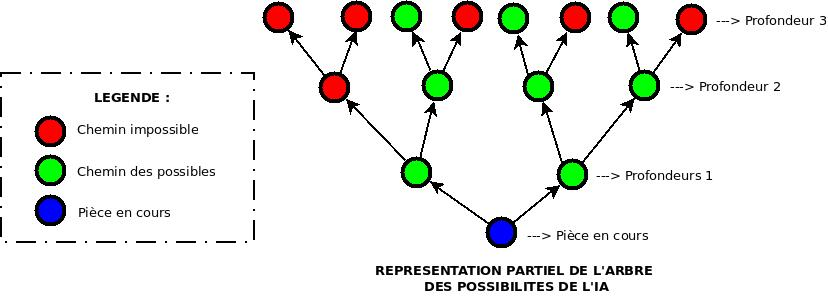
\includegraphics[width=16cm, height=8cm]{ressources/rapport/arbre_IA.jpeg} \\
            \textbf{Figure 2 :} exemple d'arbre des possibilités, avec élagage alpha-bêta.
        \end{center}
        \vspace{1cm}
        La fonction d'évaluation d'un jeu pour l'IA se base sur un algorithme simple : pour chaque ligne, pour chaque colonne et pour chaque diagonale, on regarde si trois pions sont 
            alignés avec un espace libre, et ce pour chaque joueur. On retourne ensuite une priorité associée, haute si c'est l'IA qui aligne trois pions, basse sinon. Si aucun joueur 
            n'aligne trois pions, on recommence avec deux.


%%%%%%%%%%%%%%%%%
% RÉSULTATS     %
%%%%%%%%%%%%%%%%%
\chapter{Résultats} % (3 page min)
    \paragraph*{} % bilan des objectifs
    Les objectifs principaux ont été remplis, mais d'autres, secondaires, n'ont pas bénéficié de suffisemment de temps pour être implémentés. De plus, certains aspects du programme 
        auraient gagnés à être travaillé plus avant, telle que l'architecture MVC.
        \subparagraph*{} % objectifs principaux
        Le jeu est jouable, avec quelques fonctionnalités intéressantes. Il correspond au cahier des charges, en incluant quelques suppléments, tels que le scoring.
        Ainsi, le programme propose la sauvegarde et le jeu du puissance 4 amélioré, deux fonctionnalités obligatoires pour la réussite du projet.
        \subparagraph*{} % objectifs secondaires
        Néanmoins, l'équipe aurait apprécié le développement de certains modules, dont le module graphique utilisant la SDL, ainsi que pour le son, et le réseau. Ces modules n'ont 
            pourtant pas été développés, suite à un manque de temps en fin de projet (voir paragraphe suivant). Ils seront peut-être développés plus tard, en dehors du projet, 
            pour le plaisir des développeurs désireux de découvrir (ou de redécouvrir) la SDL et ses nombreux modules.
        En outre, beaucoup de modules n'ont pas été suffisemment travaillé. le oteur, notamment, avec une sauvegarde non protégée contre la corruption.
        L'Intelliegcne Artificielle à été un grand échec du projet. Elle devait être présente, mais des problèmes incompréhensibles et restés sans solutions pendant des heures de 
            recherche n'ont pas permis l'élaborationde  ce qui aurais pu être un point notoire du projet.
        \subparagraph*{} % architecture MVC
        L'architecture MVC n'est pas parfaite : en effet, le module graphique est directement dépendant du module moteur (notamment pour les structures de données jeu, joueur et action).
        Il eu fallut créer une structure propre au module graphique, ne possédant que les valeurs nécessaires, et que le main saurais créer à partir de la strcuture de jeu, auquel le
            module graphique n'aurais jamais accès. \\
        Cela aurais également permis d'améliorer l'encapsulation des données, puisqu'actuellement rien n'empêche les modules recevant la structure de jeu de la modifier.
    \newpage
    \paragraph*{} % planning 
    Dans l'ensemble, le projet à suivis une évolution habituelle pour un projet : les premières semaines ont été très rythmées, puis l'évolution a ralentit, 
        pour réaugmenter significativement dans les dernières semaines. Suite à des retards sur le moteur, qui aurais dû être finit rapidement, le programme n'est opérationnel que depuis
        quelques semaines. Certains modules n'ont pu être testés qu'à ce moment, d'où de grosses révisions de code qui ont ralentit le développement des autres modules. \\
        Néanmoins, le projet s'est terminé, même si certains objectifs secondaires n'ont pas été remplis, faute de temps. En effet, celui-ci a manqué en fin de projet. \\
        Le planning n'était pas réellement explicité. Une \textit{todo list} a été mise en place, mais aucune notion du temps ne fût explicitement utilisée; personne n'en a eu besoin, 
        le projet avançais sans avoir besoin de \textit{deadlines}. Du moins jsuqu'aux derniers jours où il s'avérait que beaucoup de détails de dernière minutes nécessitait bien
            plus de temps que prévu.
    \paragraph*{} % image
        \begin{center}
            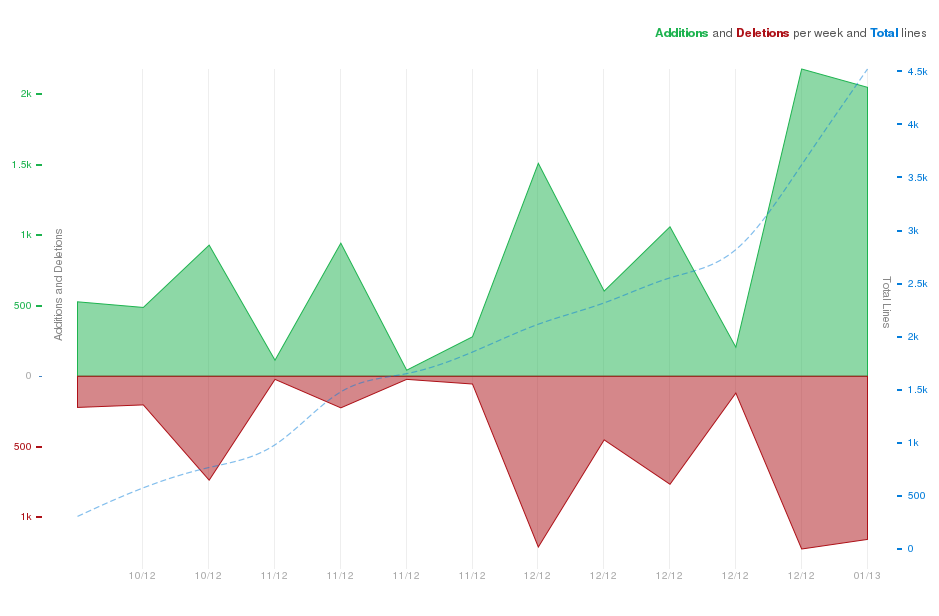
\includegraphics[width=15cm, height=11cm]{ressources/rapport/commit.png} \\
            \textbf{Figure 3 :} graphique des insertions/délétions fournit par github.
        \end{center}
        \newpage
    \paragraph*{} % améliorations 
     Pour ce projet, nous aurions aimé ajouter un module réseaux car il n'est pas très pratique de jouer à 6 devant le même ordinateur. Si le Terminal à ses limites, le bureau aussi !\\
     Nous aurions aussi aumé ajouter une interface graphique SDL. Cela nous aurait notament permis de nous affranchir de la limite des 6 joueurs grâce à beaucoup d'autre procédé : \\
     \begin{itemize}
     	\item plus de couleurs disponible;
	\item plus de formes pour les pièces;
	\item superposition moins simpliste des pièces CREUSE et PLEINE;
     \end{itemize}
     Evidemment, ne pas avoir su finir le module IA suffisemment tôt est un échec assez désagréable.
     Un autre regret : nous n'avons pas profité de ce projet pour apprendre à utiliser \textit{gdb}, bien que tout se prêtait à son utilisation, et intégration dans vim. 
        Le debuggage "à la main" était visiblement suffisant, mais se forcer à utiliser un debuggeur eût été formateur et productif.
    \newpage
    \paragraph*{} % apport du projet 
    \begin{quotation}
        Pour ma part, ce projet a été l'occasion d'approfondir mes connaissances en programmation, d'utiliser pleinement des outils comme vim, git. 
        Le fait de devoir travailler en binôme m'a montré que le celui-ci requiert une certaine rigueur, mais qu'il est plaisant de pourvoir partager ses connaissances et de reçevoir en retour. De plus nous étions tout deux de fervant utilisateurs de LINUX, ce qui nous permis de partager plus facilement nos outils. 
        Ce que je retiendrais du projet en terme de programmation sera bien evidement la programmation modulaire. Séparer chaque traitement en une fonction, et les imbriquer ensemble afin d'obtenir un ensemble cohérent. Je pense qu'un projet de ce type manquera au prochain semestre. \\ \\
        Thomas HUBA.
    \end{quotation}
    \vspace{2cm}
    \begin{quotation}
        Le projet fût assez simple dans l'ensemble, ce qui permettait de se concentrer sur un aspect résolument nouveau : le travail en binôme. 
        Rien d'évident, cela prend beaucoup de temps, pour s'y faire, entre autre à cause d'habitudes différentes, il deviens néanmoins très productif après un temps d'adaptation. 
            Plus que jamais, le gestionnaire de version est utile, ce n'est plus un simple dépôt à backup ! \\
            Certains outils sont (parfois volontairement) passés à la trappe, (debuggeur, redmine) au profit d'autres qui ont été utilisés pour le plaisir de les découvrir 
                (notamment \LaTeX). \\
            Le projet a été l'occasion d'apprendre des choses, non nécessairement en lien avec le C, comme la programmation système, la maîtrise d'environnement, 
            voir même le changement de distribution Linux pour ma part, mais participant au projet en touchant à son environnement.
            Néanmoins, ce projet terminé, cela me laisse le champs libre pour travailler sur des projets personnels chronophages, et pourquoi pas, cette fois-ci, 
                inviter d'autres personnes à me rejoindre pour réitérer l'expérience de développement en groupe. \\
            \\ \\
        Lucas BOURNEUF.
    \end{quotation}



\end{document}
% END
